\clearpage
\section{Conditional physics: observables before interpretation}
\label{sec:physics}
\subsection{Three branches that require separate assumptions}
The inspected Theory of Everything records do not specify one empirically completed model. The dated 6,433-page corpus audit identifies a controlled front packet and a Part 0 scalar-modulated open-system effective theory, followed by substantial historical and exploratory material \cite{toeaudit}. A later quadratic Higgs-portal note supplies a microscopic conditional decoherence calculation \cite{portal}. The October 22 scalar/anomaly and exact-mode packages study a specified spectral action \cite{scalar,exact}. Historical Born-bias formulas, classical rate modulation, a quadratic quantum bath, and a compactification calculation must not be combined by identifying symbols that happen to have similar names.

For clarity, write the classical modulator as $\mathcal E$, the bath field as $\varphi$, the Higgs field as $H$, and the spectral scalar amplitudes as $h_i$. A map among these objects would need a common action, symmetry assignments, dimensions, state, normalization, and matching calculation. No such full map is established in the inspected records. The connection to Quiet Calculus P10 and P22 is precisely to preserve that boundary.

\subsection{Classical rate modulation and an information-null test}
The rate branch posits a local classical response
\begin{equation}
 \gamma_k(x)=\gamma_{k0}\exp[\eta_k\mathcal E(x)],\qquad
 (\Box+m_{\mathcal E}^{2})\mathcal E=J.
 \label{eq:rate}
\end{equation}
Here $\eta_k\mathcal E$ is dimensionless and $J$ must be a physically defined source with units and a transfer function. A hidden-sector choice $J=\kappa_{\mathcal E}S^2$ appears as a working model, not a measured source. Positive continuous composition $F(a+b)=F(a)F(b)$ with $F(0)=1$ implies $F(a)=e^{\eta a}$ by applying the continuous additive functional equation to $\log F$. This conditional derivation does not establish why physical sources should compose that way.

The usual completely positive Markovian generator provides a framework for rates and specified channel operators \cite{lindblad}. Local factorization and retarded classical controls can support the sufficient no-signaling result in the dated research packet. They do not supply a unique relativistic completion or make arbitrary state-dependent nonlinear evolution acceptable.

\begin{proposition}[No information in discarded-time population bits]
\label{prop:bits}
Suppose independent identically prepared two-path probes undergo only pure dephasing in the measured path basis, with equal initial path populations. If an observation retains exactly $N$ path-basis bits and discards all timing, every bit string has probability $2^{-N}$ independent of the dephasing parameter $\lambda$. Its classical Fisher information about $\lambda$ is zero.
\end{proposition}
\begin{proof}
With $Z=\operatorname{diag}(1,-1)$, choose the convention
\begin{equation}
 \dot\rho=\frac{\lambda}{2}(Z\rho Z-\rho).
\end{equation}
Then $\dot\rho_{00}=\dot\rho_{11}=0$ and $\rho_{01}(t)=e^{-\lambda t}\rho_{01}(0)$. Each path-basis outcome remains Bernoulli$(1/2)$, and independence gives $P_\lambda(\boldsymbol x)=2^{-N}$. Consequently $\partial_\lambda\log P_\lambda(\boldsymbol x)=0$, and its squared expectation is zero.
\end{proof}

The proposition does not claim that every measurement basis is insensitive. Recombination converts coherence to an output probability. In an ideal interferometer with known phase $\theta$,
\begin{equation}
 p_+(\lambda)=\frac{1+V\cos\theta}{2},\qquad
 V=e^{-\lambda\tau},\qquad
 \mathcal I_1(\lambda)=
 \frac{\tau^2V^2\cos^2\theta}{1-V^2\cos^2\theta}.
 \label{eq:fisher}
\end{equation}
This expression assumes $0<p_+<1$ and known ideal baseline visibility. It is nonzero away from insensitive phases. In a real experiment, uncertain reference contrast, phase drift, and detection efficiencies are nuisance parameters that reduce identifiable information. Likewise, counts in a fixed duration could inform a \emph{separately specified} event rate; pure dephasing alone does not imply that event-count model.

The dated GATE-04 packet accordingly retires a fixed-count QRNG Born-bias endpoint for the rate-only branch \cite{gate04}. A biased count cannot uniquely support that branch, and an unbiased count does not constrain its rate. This is an explicit negative prediction and a useful design exclusion, not a failure to find an exotic signal. Five apparatus objects remain unspecified in that packet: source calibration, source-to-observable transfer, channel operators, nuisance likelihood, and an accessible effect/power interval.

\subsection{Quadratic portal: a conditional, dimensionally explicit bridge}
Use natural units $\hbar=c=k_B=1$. In the symmetric scalar portal convention
\begin{equation}
 V\supset\frac{\kappa_p}{2}\varphi^2H^\dagger H,
 \qquad H=\frac{1}{\sqrt2}\binom{0}{v+h},
\end{equation}
tree-level low-momentum Higgs exchange produces
\begin{equation}
 \mathcal L_{\rm eff}=c_f\varphi^2\bar f f,
 \qquad c_f=\frac{\kappa_pm_f}{2m_h^2},
 \qquad c_N=\frac{\kappa_pf_Nm_N}{2m_h^2}.
 \label{eq:portal}
\end{equation}
Here $f_N$ is the specified nucleon scalar form factor, and $c_N$ has mass dimension $-1$. The scalar-singlet literature supplies a conventional particle-physics context for portal constraints \cite{athron}; its dark-matter abundance and likelihood assumptions must not be imported into a laboratory bath without justification. The local note's symmetric interaction changes the scalar's effective mass in matter. It does not create an additive source from zero field or establish a populated bath.

Assume a free massive homogeneous Gaussian scalar bath at temperature $T$, zero chemical potential, weak coupling, two heavy fixed probe paths separated by $r$, negligible recoil, and the leading Markov limit. The connected zero-frequency noise of the renormalized composite $[\varphi^2]_R$ gives \cite{portal}
\begin{align}
 S(0,r)&=\frac{1}{2\pi^3}\int_m^\infty d\epsilon\,
 (\epsilon^2-m^2)n_\epsilon(1+n_\epsilon)
 \operatorname{sinc}^2\!\left(r\sqrt{\epsilon^2-m^2}\right),\\
 n_\epsilon&=(e^{\epsilon/T}-1)^{-1},\qquad
 \gamma(r)=c_N^2[S(0,0)-S(0,r)],\qquad
 \frac{V}{V_{\rm ref}}\simeq e^{-\gamma(r)\tau}.
 \label{eq:noise}
\end{align}
We use $\operatorname{sinc}u=\sin u/u$, continuously extended at zero. The noise has mass dimension $3$, so $c_N^2S$ is a rate. Ordinary collisional decoherence is an essential competing mechanism, not evidence of this particular portal \cite{hornberger}.

Set $a=m/T$, $b=rT$ and define $K(a,b)=\gamma/(c_N^2T^3)$. Then
\begin{equation}
 K(a,b)=\frac{1}{2\pi^3}\int_a^\infty
 \frac{(x^2-a^2)e^x}{(e^x-1)^2}
 \left[1-\operatorname{sinc}^2\!\left(b\sqrt{x^2-a^2}\right)\right]dx.
 \label{eq:kernel}
\end{equation}
The integrand supplies the exact conditional constraints
\begin{equation}
 K(a,0)=0,\qquad 0\le K(a,b)\le K_\infty(a),\qquad
 K_\infty(a)=\frac{-a\ln(1-e^{-a})+\operatorname{Li}_2(e^{-a})}{\pi^3}.
\end{equation}
For fixed $a>0$, small separation gives
\begin{equation}
 K(a,b)=\frac{b^2}{6\pi^3}\int_a^\infty
 (x^2-a^2)^2\frac{e^x}{(e^x-1)^2}\,dx+O(b^4).
\end{equation}
Thus $\gamma(2r)/\gamma(r)\to4$ as $rT\to0$ at fixed state. At large separation the rate approaches $c_N^2T^3K_\infty$, and for $m/T\gg1$,
\begin{equation}
 \gamma(\infty)\simeq\frac{c_N^2}{\pi^3}(mT^2+T^3)e^{-m/T}.
\end{equation}
The massive-bath zero-frequency rate vanishes as $T\to0$ under these assumptions; finite switching transients are outside that assertion. A general monotonicity claim is unnecessary because the sinc kernel oscillates. Equal mean fields on two paths also do not imply zero difference noise.

\begin{figure}[htbp]
\centering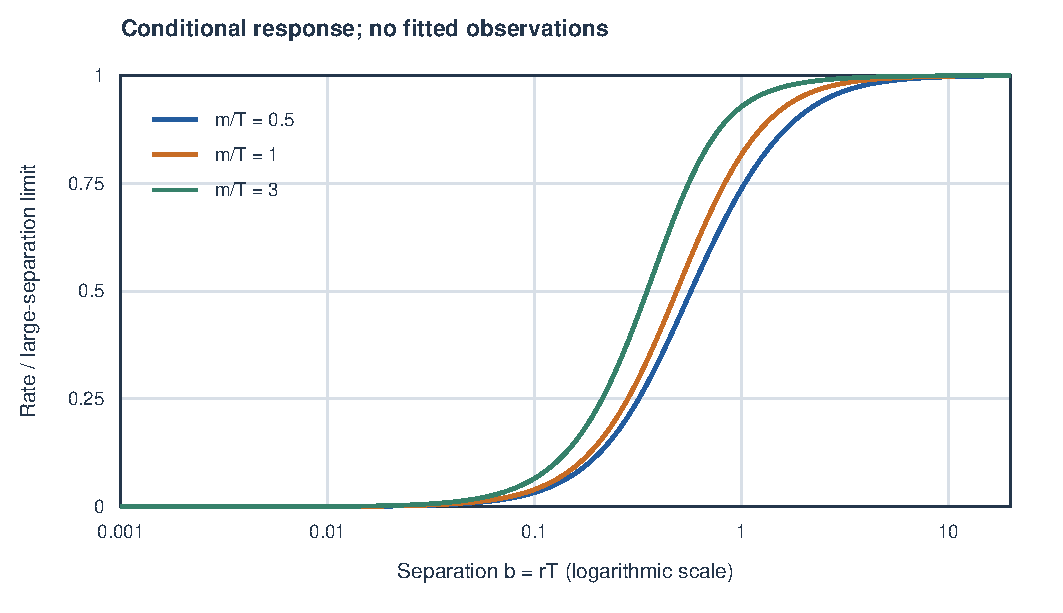
\includegraphics[width=.96\linewidth]{figures/portal_shape.pdf}
\caption{New deterministic illustration of Eq.~\eqref{eq:kernel}: normalized separation response at prescribed $m/T$. Curves are conditional calculations with no fitted data or laboratory amplitude. The small-separation slope is quadratic and the large-separation limit is one. The accompanying JSON records quadrature convergence checks.}
\label{fig:portal}
\end{figure}

For the same prepared bath and probe, ratios of nonzero rates at two separations cancel $c_N^2$. The ratio is undefined at zero coupling or zero reference rate, and its measurement becomes ill-conditioned near that limit. Composite probes require form factors and full path histories; the point-nucleon curve cannot simply be multiplied by a mass-squared factor for an arbitrary apparatus.

\subsection{Cross-channel matching and identifiability limits}
If $m<m_h/2$, the same convention gives
\begin{equation}
 \Gamma_{h\to\varphi\varphi}=\frac{\kappa_p^2v^2}{32\pi m_h}\beta,
 \qquad \beta=\sqrt{1-4m^2/m_h^2}.
\end{equation}
Eliminating $\kappa_p^2$ yields the conditional cross-channel relation
\begin{equation}
 \gamma_N(r)=\frac{8\pi f_N^2m_N^2}{v^2m_h^3\beta}
 \Gamma_{h\to\varphi\varphi}\,[S(0,0)-S(0,r)].
 \label{eq:cross}
\end{equation}
An invisible-width constraint applies only if the daughter particles are invisible in the relevant analysis and its production/width assumptions are satisfied. This paper inserts no numerical collider limit and performs no joint fit. The bath population remains an independent physical input: an upper bound on the coupling does not impose a positive lower bound on laboratory decoherence.

Identifiability is the central difficulty. In Eq.~\eqref{eq:rate}, the transformation $\mathcal E\mapsto A\mathcal E$, $\eta\mapsto\eta/A$ leaves the rate unchanged unless the source scale is independently calibrated. In Eq.~\eqref{eq:noise}, unknown occupation can trade against coupling strength. Shape measurements can constrain some combinations but do not recover all microscopic parameters. A shared fitted damping curve is compatible with several ordinary environmental models. A discriminating analysis needs independent state information, variation of separation and duration, conventional background measurements, and a frozen nuisance likelihood.

\subsection{Exact spectral calculations: approximation control and symmetry}
The scalar/anomaly and exact-mode packages define a separate parity-even classical spectral action \cite{scalar,exact},
\begin{equation}
 S_{\rm sp}=\frac{\kappa_s}{2}\operatorname{Tr}_{\rm Dirac}
 f(D_6^2/\Lambda^2),\qquad
 f(z)=\sum_a w_ae^{-az},\quad a,w_a>0,\quad\sum_aw_a=1.
\end{equation}
The stated geometry is a round internal sphere with $R=\Lambda r$, prescribed monopole sectors and four copied repaired Weyl blocks. Opposite six-dimensional chiralities are inherited assumptions. The geometric weak lift retains its Pauli/curvature vertex. The scalar convention uses $\Phi_i=r^{-1}H_iY_{1/2}$ and $h_i=H_i/(\Lambda R)$; bare amplitudes $h_i$ are not canonical physical vacuum expectation values.

Two admissible profiles share six retained local quantities but differ in exact finite-radius response. At the prescribed $R_*=1.2784724120\ldots$, four blocks, unit dimensionless Yukawas, and profile $f_-$, the saved exact coefficients are
\begin{align}
 C_0&=1.3093131218\times10^{-4},&
 C_1&=2.0841549984\times10^{-4},\\
 C_0+C_1&=2A_4,& C_1/C_0&=1.5917926458\ldots .
\end{align}
The local $a_2$--$a_4$ approximation instead gives $C_0=C_1=1.9351057742\times10^{-4}$. A parallel-flavour identity protects their sum, not their equality. The exact low-momentum quadratic parameter $2A_2/G=-1.7615373631\ldots$ differs from the local $-1.4901575034\ldots$ by about 18.21\% in magnitude. It is not a computed pole mass. These results make P10 and P22 concrete: preserving selected summaries does not identify the full response.

For neutral aligned backgrounds the stipulated charge $Q=J_3+q_Y$ commutes with the background operator. Consequently the neutral mass matrix satisfies
\begin{equation}
 M^2N=0,\qquad N=(1,1,0)^T,\qquad e^{-2}=N^TKN,
\end{equation}
where $K$ is the neutral kinetic matrix and the other directions are assumed massive. A pure-$X$ St\"uckelberg term preserves that direction. At the fixed $f_-$ fixture,
\begin{equation}
 \frac{e^{-2}}{\kappa_s}=0.3999904283
 -0.03932044965h_d^2-0.03773847661h_u^2+O(h^4).
\end{equation}
The difference between the unbroken profiles is $1.5519080\times10^{-7}$, or approximately $3.87986\times10^{-7}$ relatively. This compares mathematical profiles at a fixed bare fixture; it is not a predicted temporal variation of the measured fine-structure constant. The exact continuation also corrects the predecessor's weak-kinetic claim: its geometric $WW$ Higgs correction already has an $a_4$ curvature contribution, rather than first appearing at $a_6$.

The exact bundle records 126 passing checks and its twenty-two manifest entries match. Those are saved computational checks and current file-integrity findings, not 126 experiments. A consistency identity preserved by many theories cannot uniquely confirm this spectral construction.

\subsection{A coupled-vacuum gate and a candidate running observable}
The earlier local scalar fixture found no flat stationary radius within its sampled interval $0.1\le R\le30$ or its stated asymptotic analysis, but its scalar minimum also violated its expansion domain. The exact continuation evaluates fixed-radius coefficients and does not solve a replacement coupled vacuum. Therefore neither record supplies a physical vacuum for the entire proposed completion.

A valid gate must solve joint stationarity and flatness in a declared truncation, remove gauge directions, require positive physical kinetic eigenvalues, and test the kinetic-normalized Hessian for unwanted instabilities. It must also calculate the six-dimensional anomaly polynomial and actual two-form reduction: cancellation among four-dimensional zero modes does not prove higher-dimensional consistency. Failure rejects the specified completion, not every possible theory using similar vocabulary. A bounded numerical search must remain labeled bounded unless supplemented by analytic or interval guarantees.

The saved charge bookkeeping gives the one-loop coefficients
\begin{equation}
 (b_3,b_2,b_Y,b_X,b_{YX})=
 \left(-\frac{17}{3},-\frac53,\frac{83}{9},\frac{316}{3},0\right).
\end{equation}
Under exactly that active matter content, charge convention, and a threshold-free perturbative energy interval,
\begin{equation}
 \frac{d g_i^{-2}}{d\ln\mu}=-\frac{b_i}{8\pi^2},\qquad
 \frac{d(g_Y^{-2}-g_2^{-2})}{d\ln\mu}=-\frac{49}{36\pi^2}.
 \label{eq:running}
\end{equation}
The difference removes a constant matching offset. It does not remove dependence on particle content, thresholds, higher orders, or measured scattering inputs. Four chiral generations in the stipulated notes require an explicit phenomenology audit before this can be presented as a viable model of observed matter. No such viability conclusion is established here. Similarly, $b_{YX}=0$ for complete active multiplets does not eliminate finite mixing from unequal thresholds.

The tree-level massless CP-odd physical scalar in the stipulated two-doublet-plus-axion construction is another conditional symmetry result. QCD effects and allowed operators can lift it; an independently predicted physical mass and coupling are absent. It is a future matching problem, not a claimed detectable axion signal.
